%%==========================================================================
\section{Experiments}
\label{sec:experiments}

We have used synthetic data and real captured data to evaluate the SuperMatching algorithm.
To demonstrate  the SuperMatching algorithm's independence of feature descriptors, several descriptors were used.
In some cases, we simply uniformly sampled feature points on the objects, and used a trivial feature descriptor of 1 for all points, meaning affinities are based simply on distances between feature points---this allows us to show our method is robust in the presence of ambiguous feature descriptors.
In other cases, we still used uniformly distributed feature points, together with SIFT descriptors, which shows that feature points do not have to be carefully chosen.
We used third-order matching in our experiments, but it would be simple (but more costly) to use higher order.

%-------------------------------------------------------------------------
\subsection{3D Rigid Shapes Scans}
\label{subsec:3DRigid}

Firstly, we used SuperMatching to build pairwise matchings between 3D rigid shape scans based on uniformly sampled feature points.
Rigid transforms can be computed from each triple of compatible matching points.
The transform which brings the most data points within a threshold distance of a point in the model is chosen as the optimal alignment transform~\cite{Huttenlocher90}.
As discussed in \cite{Gelfand05}, such a voting scheme is guaranteed to find the optimal alignment between pairwise scans and is robust to the initial pose of the input scans.
Figure~\ref{fig:3DPair} shows some registration results for the Rooster model from \cite{Chuang09}. The left column shows the original state,
the two middle columns are our matching and alignment results, and
the right column shows the corresponding result produced by \cite{Aiger08}, which has clearly failed.
The transformation matrix computed by  SuperMatching is compared with the ground truth provided by \cite{Chuang09} in Table~\ref{tab:matrix},
which demonstrates that our computed matrices for matching I-II and I-III are very close to the ground truth.
Note that the matrices are used to transform and alignment from II to I and III to I transformations. 

\begin{figure}[t!]
\centering
  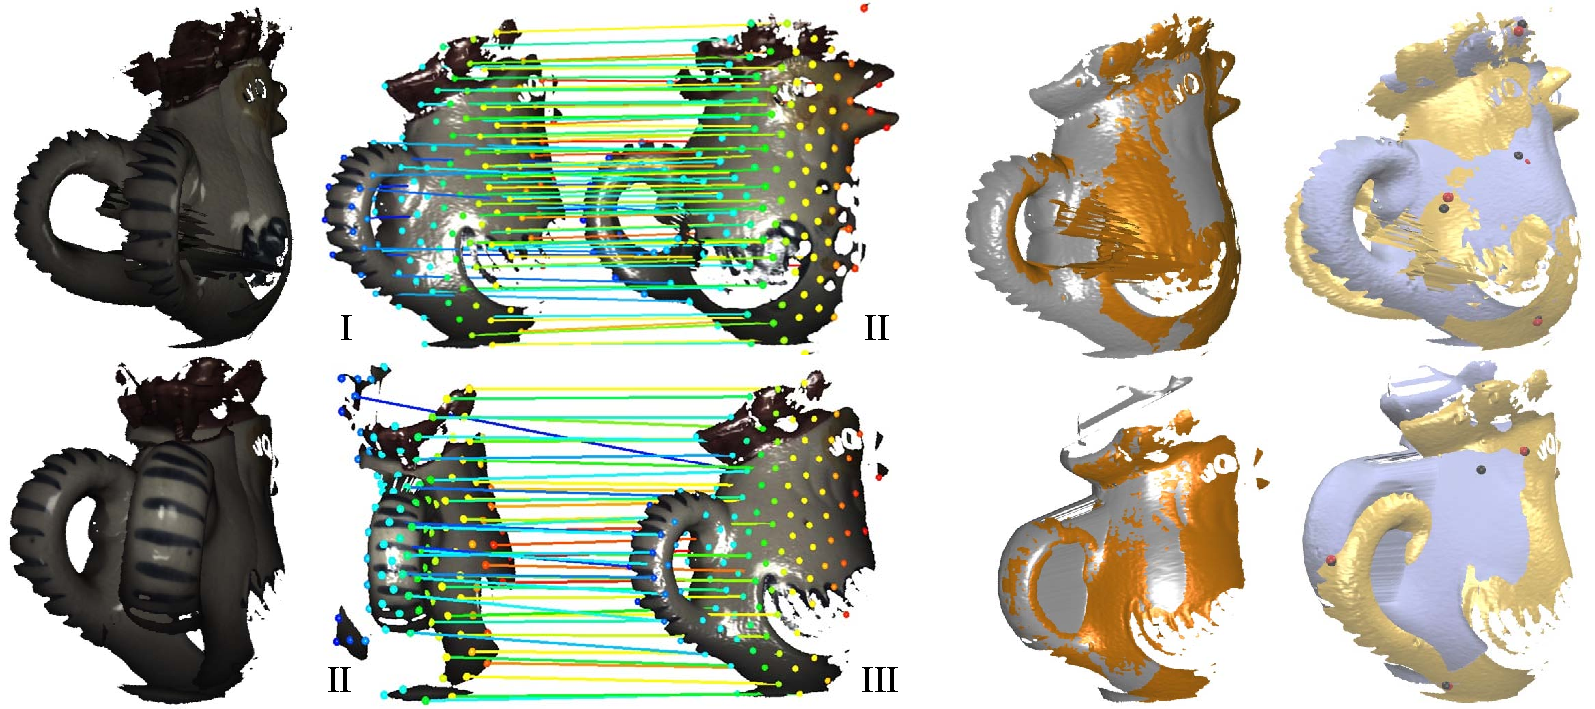
\includegraphics[width=0.99\linewidth]{figures/RoosterPair2.pdf}
  \caption{Pairwise alignment of Rooster \emph{$I-II$} and \emph{$II-III$} scans.
  From left to right: before alignment, our matching result, our alignment result, alignment result from [Aiger et al. 2008].}
\label{fig:3DPair}
\end{figure}

\begin{table}[tb]
%\vspace{-4mm}
\centering
%\renewcommand{\arraystretch}{0.8}
\tabcolsep=1pt
\setlength{\aboverulesep}{0pt}
\setlength{\belowrulesep}{0pt}
\caption{Transformation matrix comparison}
\hspace{-5ex}
\label{tab:matrix}
\small
\begin{tabular}{c |rrrr |rrrr}
\toprule
 & \multicolumn{4}{|c|}{ {computed matrix}} & \multicolumn{4}{c}{ {ground truth}} \\
\hline
{I} & {0.7298} 	& {-0.0046}   & {-0.6822}	& {-127.6}  & {0.7073} 	& {-0.0043}   & {-0.7069}	& {-132.3}   \\
%\hline
{|}&{-0.0056}     &  {1.0000}	& {-0.0155} & {-3.016}  & {-0.0116}	& {0.9998}	& {-0.0177}	& {-3.3}   \\
%\hline
{II}&{0.6928}	    & {0.0206}	& {0.70021}	& {-50.05}  & {0.7068}     & {0.02067}   & {0.7071}	& {-54.1}   \\
%\hline
&{0}             & {0}	        & {0}	        & {1}          & {0}             & {0}	        & {0}	        & {1}          \\
\hline
{I} & {0.0051} & {-0.0118} &  {-0.9948} & {-186.8}          & {0.0007} & {-0.0220} &  {-0.9998} & {-187.7}  \\
%\hline
{|}  &{-0.0139} & {1.0028} &{-0.0218} & {-4.769}  	&{-0.0322} & {0.9992} &{-0.0220} & {-4.1}   \\
%\hline
{III} &{1.0166} & {0.0362} &{0.0052} &{-176.6}       &{0.9995} & {0.0322} &{0.0000} &{-186.0}  \\
%\hline
&        {0}             & {0}	        & {0}	        & {1}          & {0}             & {0}	        & {0}	        & {1}          \\
\bottomrule
\end{tabular}%
%\vspace{-27pt}
%\vspace{-8mm}
\end{table}%


Next, we used SuperMatching to build a complete model from a set of scans from different viewpoints.
For these multiple scans, third-order matching was first performed between each pair of consecutive scans.
After doing so, the alignment was refined using the iterative closest point (ICP) algorithm \cite{Besl92}.
Figure~\ref{fig:3DRigid} illustrates the approach and shows the result.

\begin{figure}[t!]
\centering
  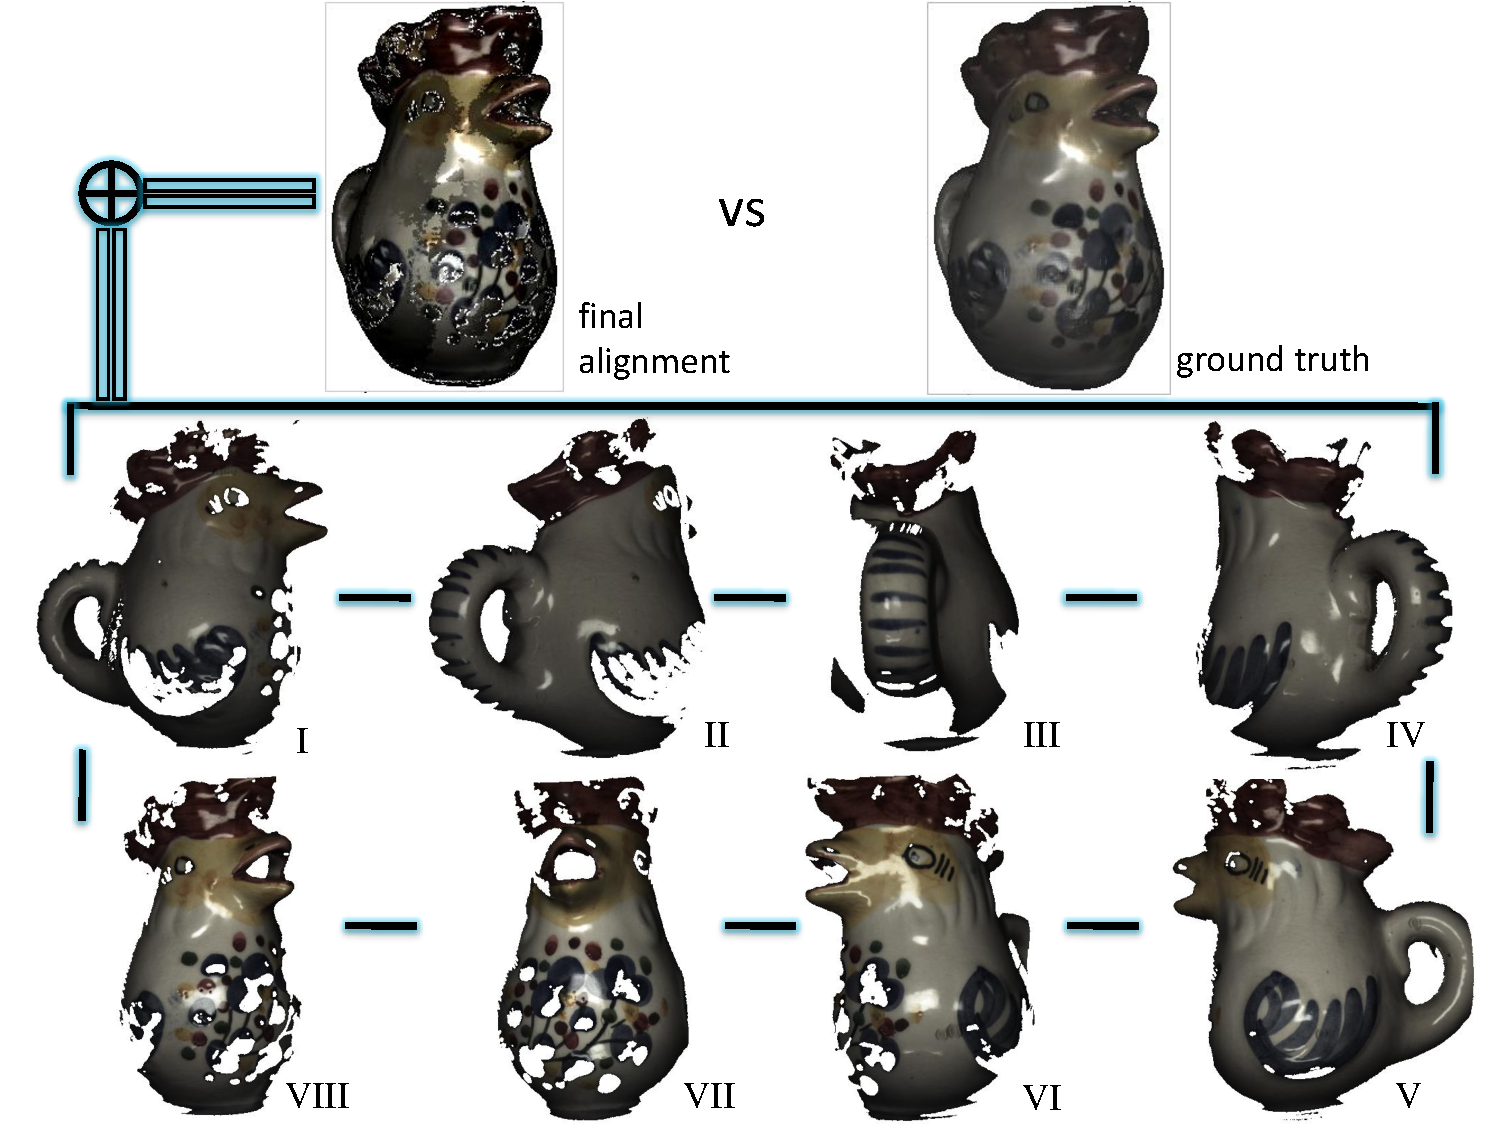
\includegraphics[width=0.99\linewidth]{figures/Rooster.pdf}
  \caption{Alignment of several Rooster scans from different viewpoints.
  Above: our final registered Rooster and the ground truth [Chuang et al. 2009]. Below: 8 partial scans, the dark lines indicating the pairwise matches.}
\label{fig:3DRigid}
\end{figure}

%-------------------------------------------------------------------------
\subsection{3D Depth Scans with Color Information}
\label{subsec:3dColored}

We next provide a further real-world, noisy, example of the use of SuperMatching.
In this case, data with surface color information was captured using a Kinect camera \cite{Kinect12}.
Uniform samples and SIFT feature vectors were used as a basis for SuperMatching.
This resulted in robust matches, as illustrated in Figure~\ref{fig:3DReal}.

\begin{figure}[h]
\centering
  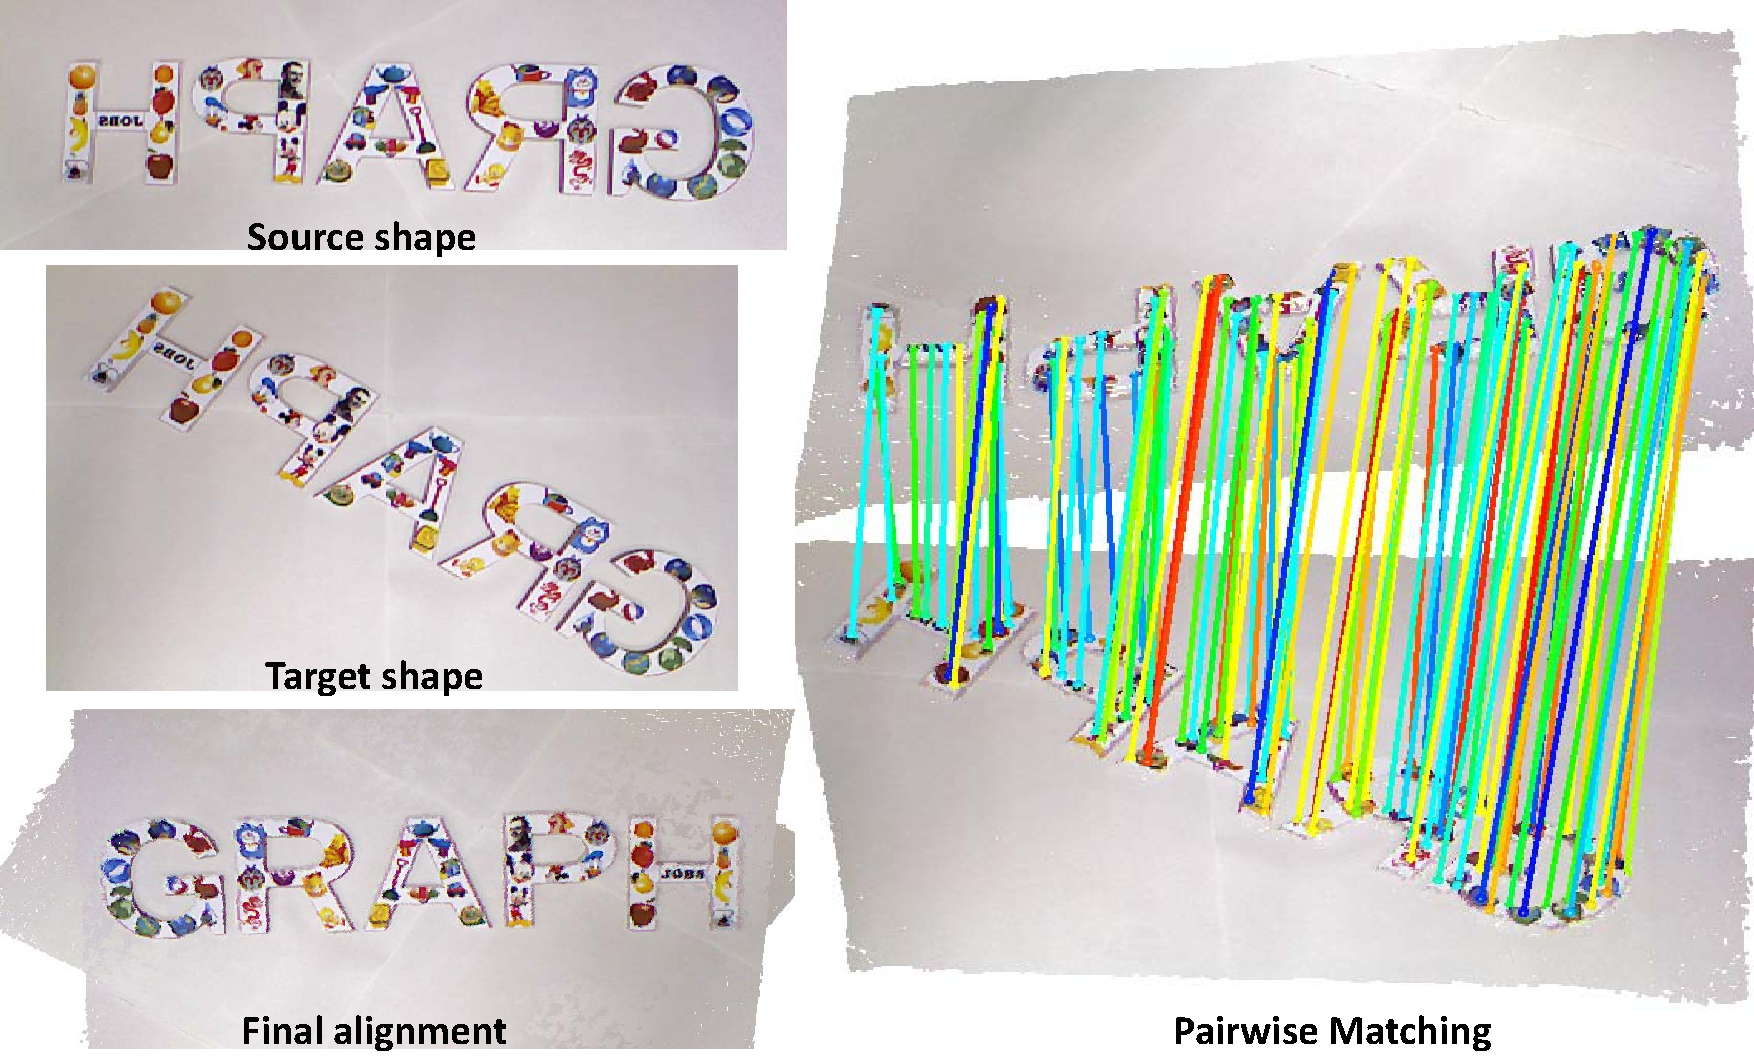
\includegraphics[width=1.05\linewidth]{figures/kinect.pdf}
  \caption{3D real depth scans with color information, captured using Kinect.
    Matching points are connected by colored lines.}
\label{fig:3DReal}
\end{figure}

%-------------------------------------------------------------------------
\subsection{3D Articulated Shape Synthetic Data}
\label{subsec:3darticulated}

A further application is registration of (approximately) articulated shapes. Such problems are common in dynamic range scanning such as human motion capture.
Given a sequence of range scans of a moving articulated subject, our method automatically registers all data to produce a complete 3D shape.
Unlike many other methods, we do not need  manual segmentation, markers, or a prior template.
While the problem of non-rigid registration of deformable shapes is ill-posed and no algorithm is applicable to all scenarios,
we believe that our approach pushes the limits of what can be achieved with minimal prior information. SuperMatching provides robust, accurate matching,
even although the partial scans have holes and different poses.

Again uniformly sampled points were used. Registration of scans was performed by computing piecewise rigid transformations between matches.
These transformations may be propagated from feature points to the entire set of points in each scan using nearest neighbor interpolation.
Figure~\ref{fig:3DRobot} shows a registration example for an articulated model.
On the left is our result, on the right is the result produced by the method \cite{Chang09}.

\begin{figure}[t!]
\centering
  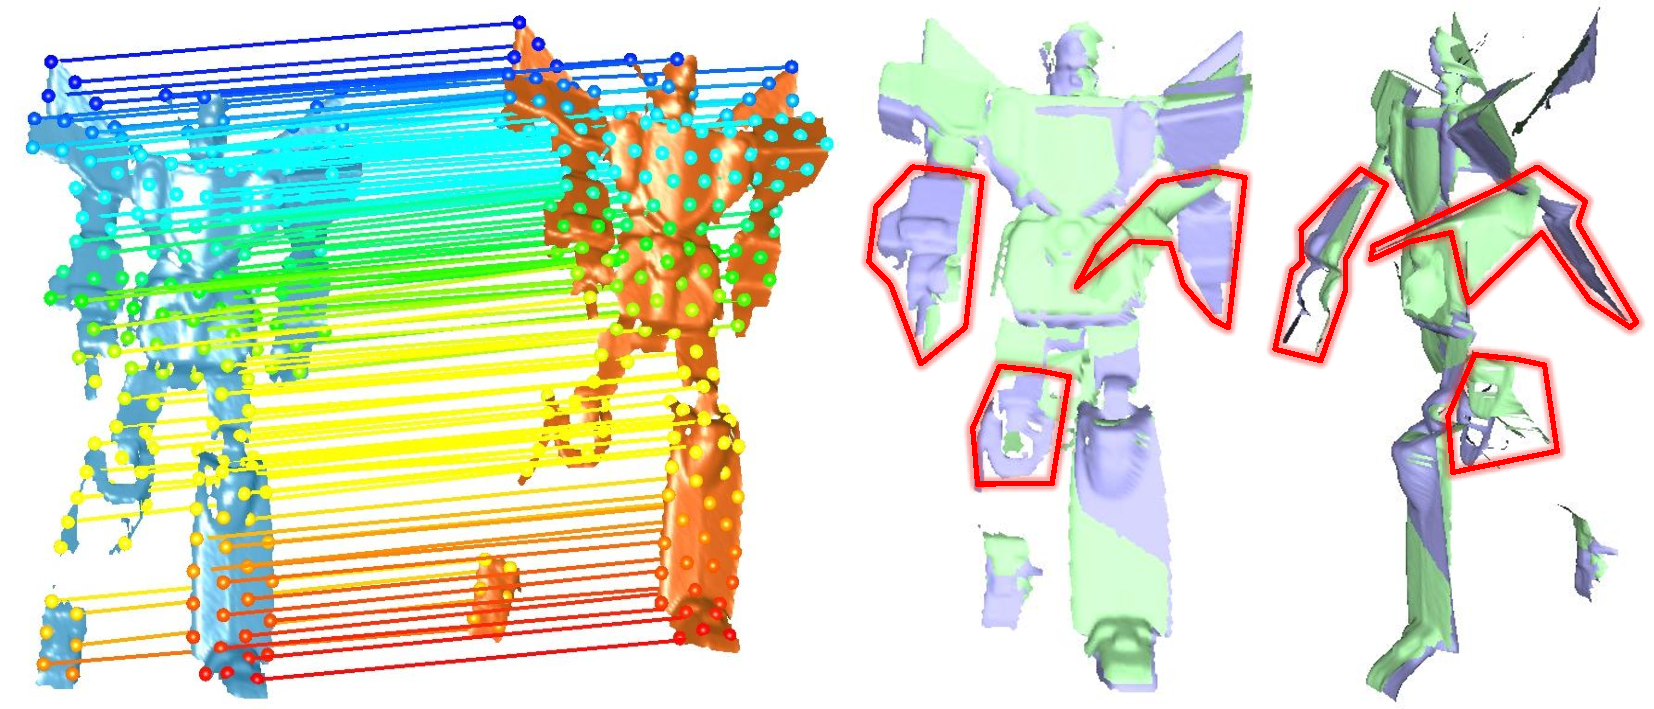
\includegraphics[width=0.95\linewidth]{figures/Robot.pdf}
  \caption{Pairwise matching of an articulated Robot between two frames.
           Left: our result. Right: result produced by [Chang and Zwicker 2009], from front and side views; red polygons indicate regions of large distortion.}
\label{fig:3DRobot}
\end{figure}

For a sequence of partial articulated data, registration is performed in two main steps.
We first precompute an initial pairwise registration for each pair of consecutive frames, then perform articulated shape reconstruction as in \cite{Pekelny08}.
Segmentation of the scans into rigid parts can readily be done by clustering the transformations obtained from uniformly feature points,
using the mean shift algorithm \cite{Comaniciu02}.
This information is used as input to the second step of articulated shape reconstruction following \cite{Pekelny08}:
this algorithm identifies and tracks the rigid parts in each frame, while accumulating  geometric information over time.
However, \cite{Pekelny08} requires the user to manually segment each range scan in advance, whereas we automatically determine  the segmentation.
Figure~\ref{fig:3DHand} shows an articulated hand example.
This synthetic data is generated from a deformation sequence, and the final registered shape is produced from these partial data.
By using synthetic data, we are able to evaluate the robustness of our reconstruction method using the ground truth, as shown in Figure~\ref{fig:3DHand}.
Quantitatively, we measured the maximum of the average distance of the reconstruction over all frames as $0.001 D$ where $D$ is the bounding box diagonal length, and
the greatest distance error in any one frame was $0.012 D$.

\begin{figure}[t!]
\centering
  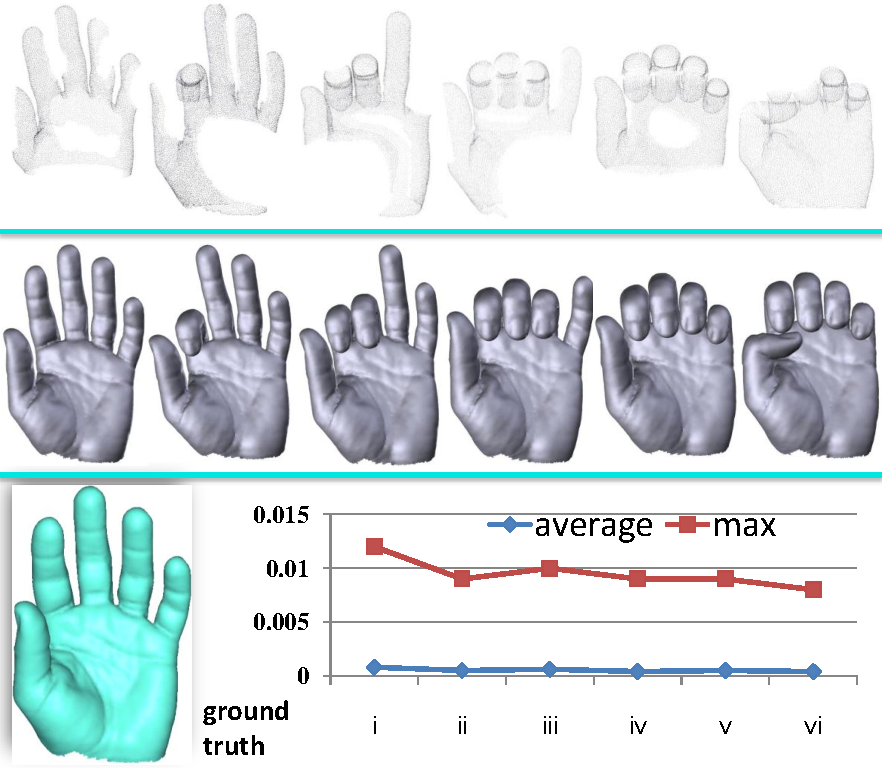
\includegraphics[width=0.95\linewidth]{figures/3DHand.pdf}
  \caption{Registration of an articulated hand.
  Above: partial synthetic data with holes generated from a deformation sequence.
  Middle: reconstructed meshes are deduced from the registration process.
  Below: first frame ground truth shape, and average and maximum distance from the ground truth per frame.}
\label{fig:3DHand}
\end{figure}

%-------------------------------------------------------------------------
\subsection{Deformable Surfaces}
\label{subsec:2DDeformable}

Finally, we matched SIFT points on images of deforming surfaces\footnote{From \url{http://cvlab.epfl.ch/data/dsr/}} showing a cloth and a cushion.
The surface of the cloth underwent relatively smooth deformation, while the surface of the cushion included sharp folds.
This data comes with ground truth, which allows quantitative verification of the accuracy of the matches found.
From each surface set we randomly chose two frames before and after a large deformation.
We randomly chose $100$ corresponding points on each surface, using the provided ground truth.

We used the above input data as a basis for comparison with the spectral algorithm \cite{Cour06} (a quadratic assignment algorithm),
a third-order tensor algorithm \cite{Duchenne09},
and the hypergraph matching algorithm \cite{Zass08}, using the authors' code in each case.
All methods were executed in Matlab on a $2.3$GHz Core2Duo with $2$GB memory.
To enable direct and fair comparison,
\cite{Duchenne09}, \cite{Zass08} and SuperMatching used the same potential and the same tensor size.

In these tests, SuperMatching considered $3\times 10^6$ feature tuples, while the method of \cite{Duchenne09} considered $10\times 10^6$ tuples  and the method of \cite{Zass08} used $4\times 10^6$.
The difference mainly results from differences in sampling strategy; note that we have the lowest  sampling cost.
The average running time to match two feature sets each with $100$ features was around 8s for SuperMatching, 13s for \cite{Duchenne09}, 6.5s for \cite{Zass08}, and 5s for \cite{Cour06}.
SuperMatching takes less time than the third-order tensor algorithm in \cite{Duchenne09} both because it uses fewer feature tuples and because of the more efficient supersymmetric higher-order power iteration solution.

Matching accuracy was assessed by the number of correctly matched points (known from the  ground truth) divided by the total number of points that could be matched.
The results are summarised in Table~\ref{tab:errorrate1} and illustrated in Figure~\ref{fig:2DDeformable}.
Table~\ref{tab:errorrate1} demonstrates that SuperMatching achieves a higher matching accuracy than previous algorithms.
The worst matching result is produced by the spectral quadratic assignment algorithm \cite{Cour06},
due to the lower discriminatory power of pairwise geometric constraints.
Higher-order algorithms perform better due to the more complex geometric constraints.
Nevertheless, SuperMatching also significantly outperforms the third-order algorithm \cite{Duchenne09} and the hypergraph matching algorithm \cite{Zass08},
as these do not tale proper advantage of supersymmetry.

%----------------------------------------
%  deformable matching results IMAGES
%----------------------------------------
%----------------------------------------
\begin{figure}[tb]
\centering
  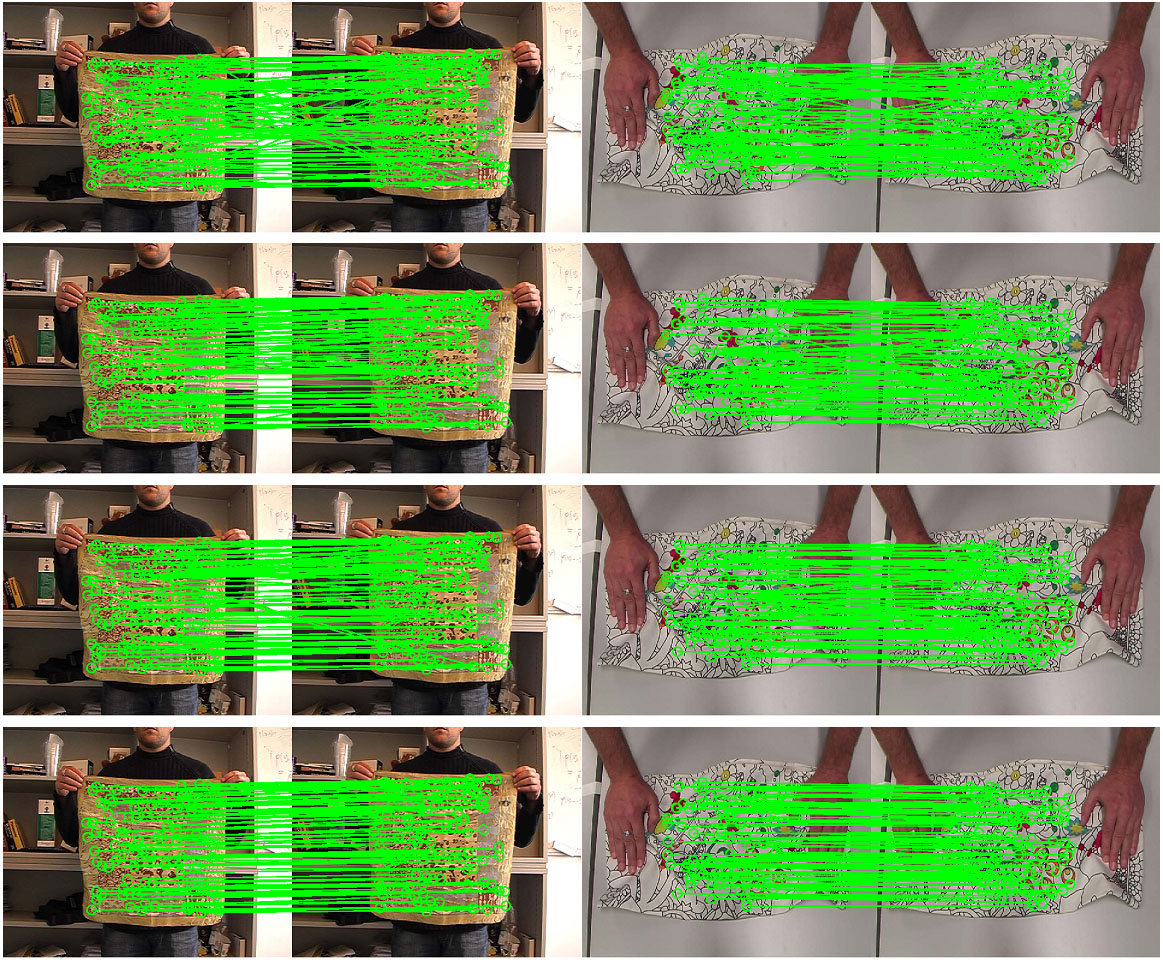
\includegraphics[width=1.00\linewidth]{figures/2DDeformable.jpg}
  \caption{Matching results. Left: cloth set, matching between frame 80 and 90, right: cushion set, matching between 144 and 156.
  Top to bottom, spectral method [Cour et al. 2006], hypergraph matching method [Zass and Shashua 2008], a third-order tensor method [Duchenne et al. 2009], and SuperMatching.}
\label{fig:2DDeformable}
\end{figure}

%%%RRM This table is too wide. Omit the last two columns
%----------------------------------------
%  deformable matching results TABLE
%----------------------------------------
\begin{table}[tb]
%\vspace{-4mm}
\centering
%\renewcommand{\arraystretch}{0.8}
\tabcolsep=1pt
\setlength{\aboverulesep}{0pt}
\setlength{\belowrulesep}{0pt}
\caption{Accuracy of deformable surface matching.}
\hspace{-5ex}
\label{tab:errorrate1}
\small
\begin{tabular}{l|c c c c | c c c c | r}
\toprule
{Dataset}  & \multicolumn{4}{|c|}{ {cloth}} & \multicolumn{4}{c|}{ {cushion}} & \\
\hline
 {Matching frames} &  {F80-}	&  {F90-}	& {F95-}	& {F100-} & {F144-} & {F156-}	& {F165-}	& {F172-} &  {Time}  \\
 {}                &  {F90 }    &  {F95 }   & {F100}    & {F105}  & {F156}  & {F165}    & {F172}    & {F188}  &  {(s)} \\
\hline
 {SuperMatching}   &  {83\%}    &  {85\%}	& {84\%} 	& {81\%}  & {66\%}	& {60\%}	& {69\%}	& {56\%}  &  {8}  \\
%\hline
 {\cite{Zass08}}   & {73\%}	    & {79\%}	& {70\%}	& {72\%}  & {44\%}  & {39\%}    & {54\%}	& {43\%}   & {6.5}  \\
%\hline
{\cite{Duchenne09}} & {67\%}    & {77\%}    & {73\%}	& {65\%}  & {39\%}	& {31\%}	& {47\%}	& {42\%}   & {13}  \\
%\hline
 {\cite{Cour06}}   & {27\%}     & {29\%}	&  {22\%}	& {27\%}  & {14\%}  & {5\%}	    & {28\%}	& {7\%}    & {5}  \\
\bottomrule
\end{tabular}%
%\vspace{-27pt}
%\vspace{-8mm}
\end{table}%
